% !TEX program = pdflatex
\documentclass[11pt,a4paper]{article}

\usepackage[utf8]{inputenc}
\usepackage[T1]{fontenc}
\usepackage{lmodern}
\usepackage{geometry}
\geometry{margin=1in}
\usepackage{amsmath,amssymb}
\usepackage{siunitx}
\usepackage{graphicx}
\usepackage[font=small,labelfont=bf,labelsep=endash]{caption}
\usepackage{booktabs}
\usepackage{physics}
\usepackage{cite}
\usepackage{hyperref}
\usepackage{float}
\hypersetup{colorlinks=true,linkcolor=blue,citecolor=blue,urlcolor=blue}

\title{Design Methodology for a Dual-Jet Hovering Disc with Concentric Air Curtains:\\
Model, Non-Dimensionalization, and Physical Assumptions}
\author{ }
\date{ }

\begin{document}

\maketitle

\begin{abstract}
This paper presents a design-oriented physical model for a hovering disc sustained by two concentric air jets:
an outer annular jet that forms an aerodynamic curtain to confine the inner flow and an inner jet that maintains the central cushion pressure.
The analysis uses a low-Mach compressible, axisymmetric core model with an anisotropic Stokes--Darcy closure to approximate the pressure and velocity fields in the cushion region.
A detailed discussion of the model's assumptions and their physical validity is provided, along with a complete nomenclature of symbols used throughout the work.
\end{abstract}

\begin{figure}[t]
  \centering
  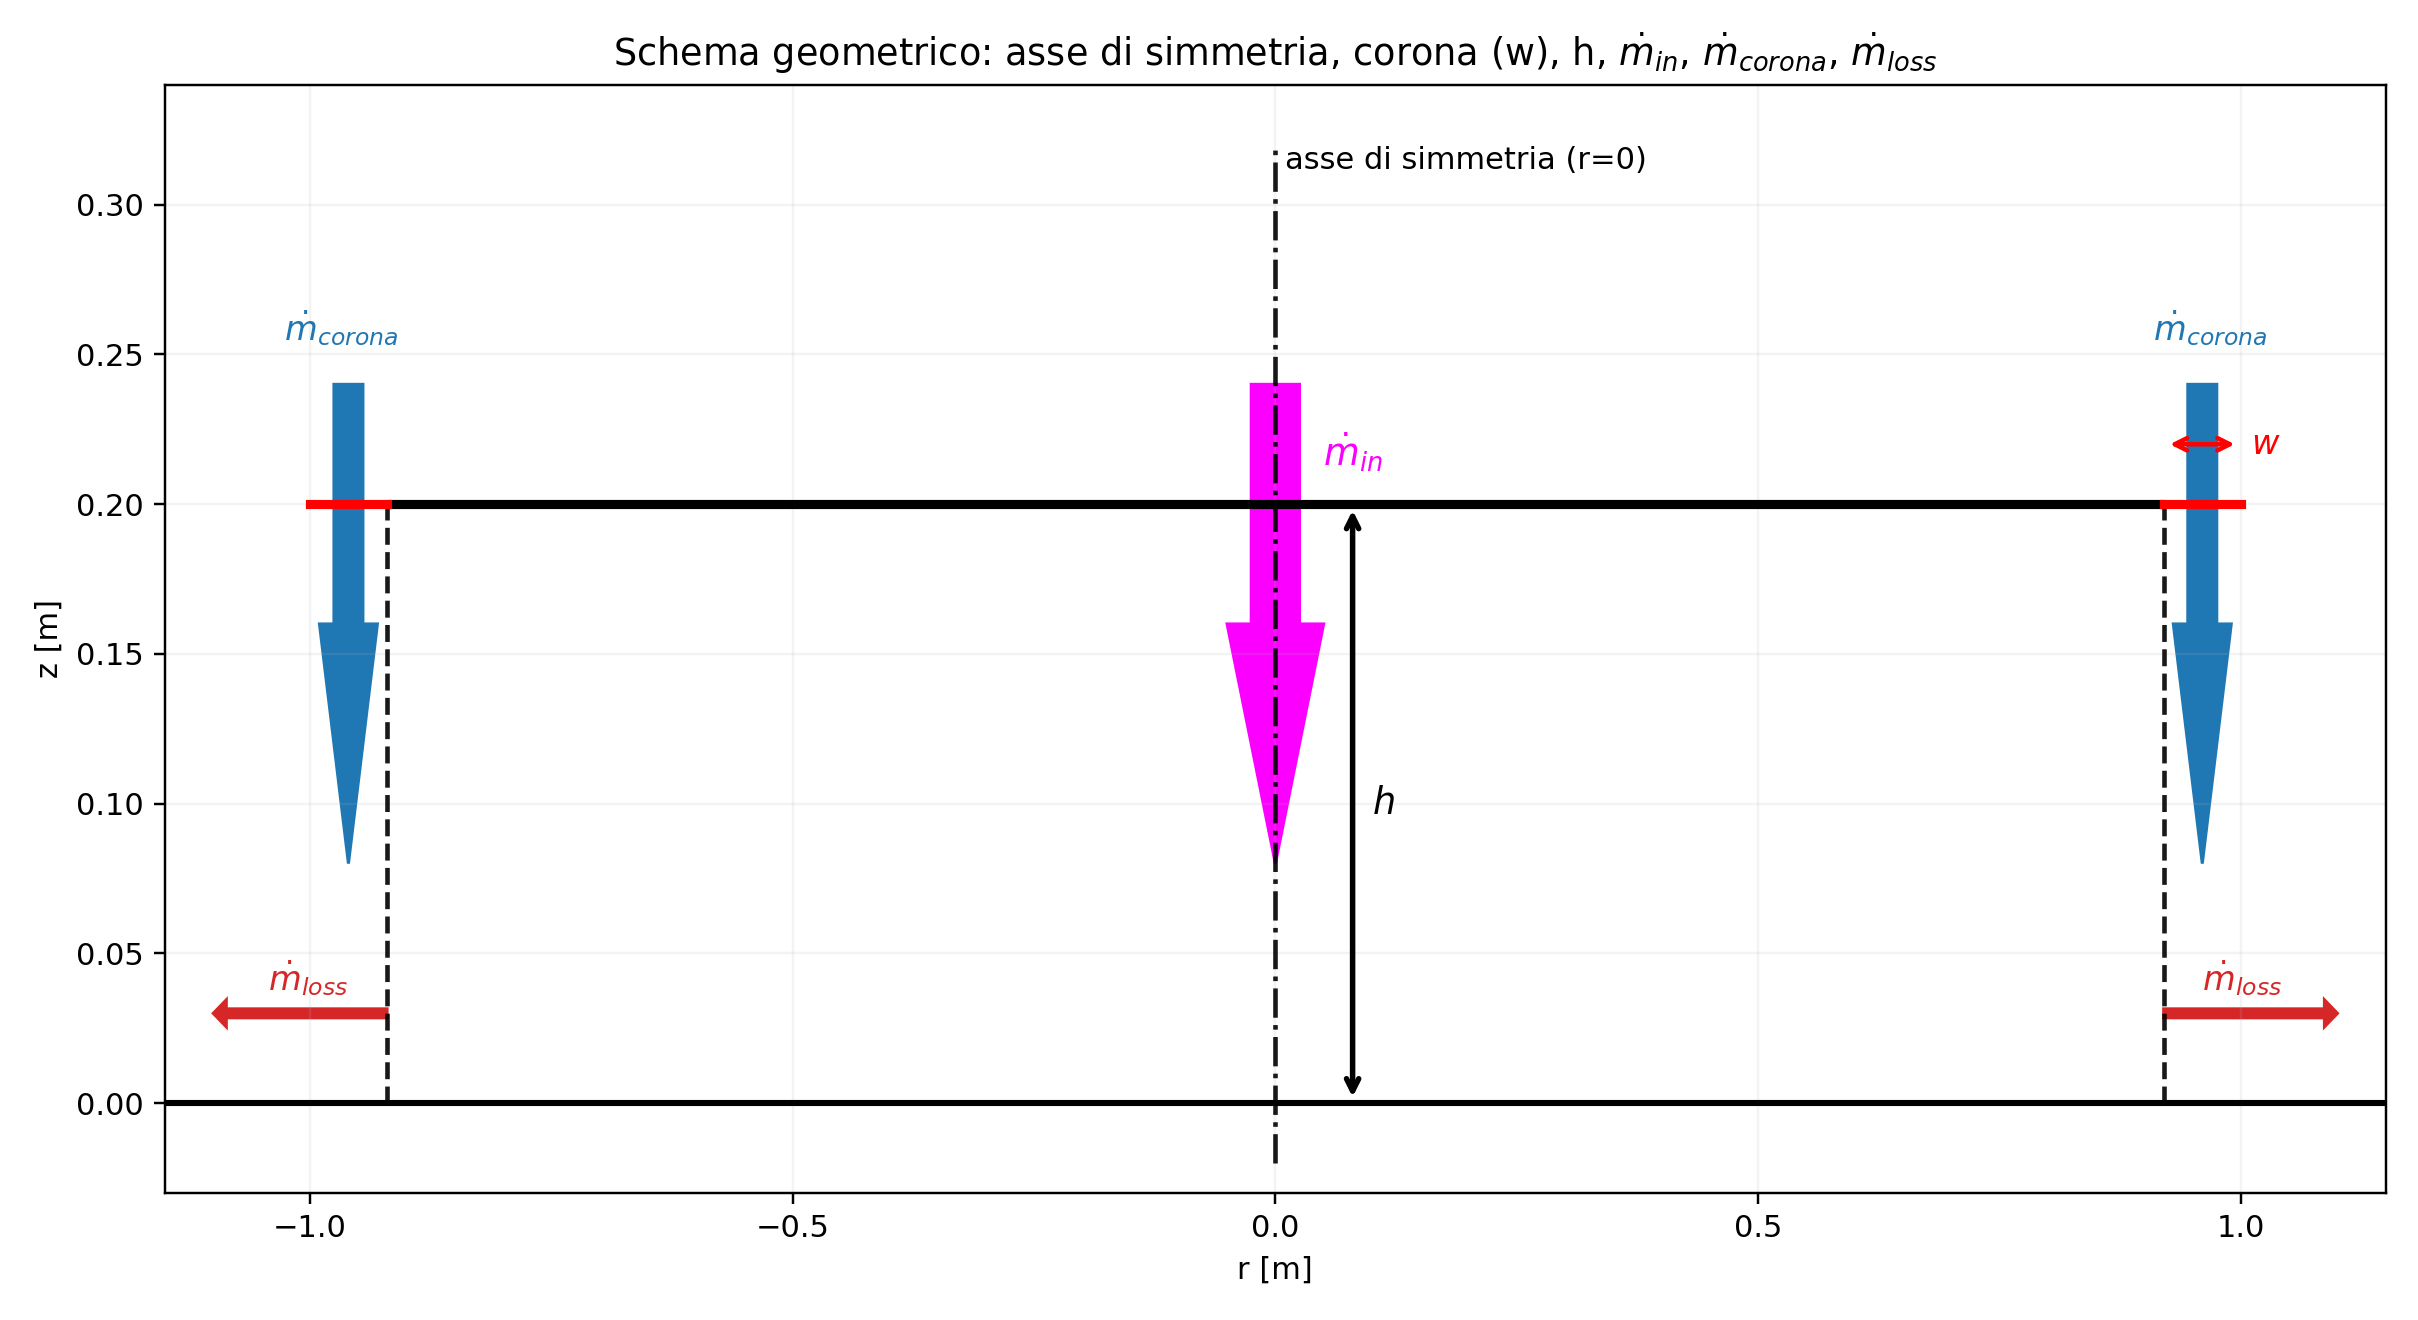
\includegraphics[width=0.95\linewidth]{../figs/schema_geometry.png}
  \caption{Schematic of the hovering disc with two concentric jets: the outer annular curtain and the central make-up flow.}
  \label{fig:geometry}
\end{figure}

\section{Geometry and Notation}
\label{sec:geometry}
The geometry follows Fig.~\ref{fig:geometry}, defining the coordinate system and characteristic dimensions:
\begin{itemize}
  \item $R_{\mathrm{tot}}$ -- total radius of the disc.
  \item $h$ -- hovering height from the ground.
  \item $w$ -- width of the peripheral leakage ring; $R^{-}=R_{\mathrm{tot}}-w$ is its inner radius.
  \item $h_{\mathrm{eff}}$ -- effective sealing height (characteristic of curtain recirculation).
  \item $p_0$ -- ambient pressure; $p_c=W/(\pi R_{\mathrm{tot}}^2)$ -- cushion pressure supporting the load $W$.
  \item $U_{\mathrm{out}}$, $\rho_j$ -- speed and density of the outer jet.
  \item $\mu$ -- dynamic viscosity; $R_g$ -- specific gas constant for air.
  \item $\dot{m}_{\mathrm{in}}$ -- air mass flow entering internal region.
  \item $\dot{m}_{\mathrm{out}}$ -- air mass flow of outer region.
  \item $\dot{m}_{\mathrm{loss}}$ -- air mass flow exiting internal region.
  \item $H$ -- effective curtain height (equal to $h$ in this study, representing the vertical extent over which the curtain resists leakage).
  \item $b_0$ -- initial slot thickness of the outer annular jet at injection.
  \item $b(z)$ -- effective local width of the curtain slot or equivalent jet region as a function of $z$ (see rim-pressure model).
\end{itemize}

\begin{table}[h]
  \centering
  \caption{Default model parameters and empirical coefficients (nominal values are exemplary and require calibration).}
  \label{tab:model-params}
  \begin{tabular}{@{}llll@{}}
    \toprule
    Symbol & Description & Unit & Nominal value \\
    \midrule
    $\alpha_r$     & Radial permeability coefficient      & —     & (e.g.\ 0.1) \\
    $\alpha_z$     & Axial permeability coefficient       & —     & (e.g.\ 0.05) \\
    $E$            & Entrainment coefficient (wall-jet)  & —     & (e.g.\ 0.3) \\
    $C_f$          & Wall friction coefficient           & —     & (e.g.\ 0.005) \\
    $k_e$          & Wall-jet thickness growth rate      & m/m   & (e.g.\ 0.01) \\
    $K_{\rm turn}$ & Momentum loss coefficient at turning& —     & (e.g.\ 1.2) \\
    $D_{m,\min}$   & Minimum deflection modulus         & —     & (e.g.\ 0.2) \\
    \bottomrule
  \end{tabular}
\end{table}

\section{Model Overview}
\label{sec:model-overview}

The cushion region ($0\le r\le R^{-},\ 0\le z\le h$) is filled with air at variable pressure, temperature, and density.
The mean flow satisfies an anisotropic Stokes--Darcy closure:
\begin{equation}
  u = -\frac{\kappa_r}{\mu}\,\partial_r p,\qquad
  w = -\frac{\kappa_z}{\mu}\,\partial_z p,
\end{equation}
with permeability coefficients $\kappa_r=\alpha_r h^2$ and $\kappa_z=\alpha_z h^2$, where $\alpha_r$ and $\alpha_z$ are empirical dimensionless parameters encoding the overall resistance of the confined air layer.

The continuity and state relations read
\begin{equation}
  \frac{1}{r}\,\partial_r\!\left(r\rho u\right)+\partial_z(\rho w)=0,\qquad
  p=\rho R_g T.
\end{equation}
Elimination of $u,w$ gives the pressure formulation:
\begin{equation}
  \frac{1}{r}\partial_r(r\rho\kappa_r\partial_r p)+\partial_z(\rho\kappa_z\partial_z p)=0.
\end{equation}




\section{Simulation Methodology}
\label{sec:simulation-method}

This section presents a clear, step-by-step procedure for simulating the coupled dynamics of the core cushion region and the outer annular curtain jet. The algorithm is designed to determine the steady pressure and velocity fields in both regions, and thereby to compute the load-carrying capacity, leakage mass flows, and power requirement of the hover system.

\subsection*{1. Domains and coupling overview}
The hover disc system is conceptually split into two interacting regions:
\begin{itemize}
  \item The \emph{core cavity}, defined by \(0 \le r \le R^{-},\;0 \le z \le h\), filled with pressurized air that supports the load and from which a peripheral leakage ring allows outflow.
  \item The \emph{outer-jet region}, comprising the annular slot at \(r=R^{-}\) through which the high-velocity curtain issues downward, impinges on the ground, and subsequently transitions into a radial wall-jet along the ground surface.
\end{itemize}
The key coupling mechanism is as follows: the outer jet impinges, creating a rim pressure distribution \(p_{\rm edge}(z)\) at the boundary \(r=R^{-}\); this rim pressure acts as a boundary condition for the core pressure field. In turn, the core pressure field determines the leakage mass flux and thus affects the required outer jet flow and velocity to maintain equilibrium.

\subsection*{2. Governing sub-problems}
\paragraph{2.1 Outer jet / curtain model}  
Given a trial outer-slot exit velocity \(U_{\rm out}\) and mass flow \(\dot m_{\rm out}\), the outer jet sub-model computes:
\begin{itemize}
  \item The impingement and turning losses at the ground (characterised by \(K_{\rm turn}\)) and the wall-jet initial conditions (speed \(U_c(r_t)\), thickness \(\delta_t\)).
  \item The integral wall-jet development from the turning radius \(r_t\) out to \(r=R^{-}\). This uses mass and momentum balances:
    \[
      \frac{d q}{dr} = E\,U_c(r), 
      \qquad
      \frac{d m}{dr} = -\tfrac12\,\rho\,U_c(r)^2\,C_f(r)
    \]
    together with a growth law for the jet thickness \(\delta'(r)=k_e\).  
  \item From the wall-jet profile, the rim pressure (seal effect) is derived in the form  
    \[
      p_{\rm edge}(z) = p_0 + \min\!\Bigg(\Delta P,\;\frac{\rho\,U(z)^2\,b(z)}{H\,D_{m,\min}}\Bigg)
      \]
    for \(0\le z\le H\). Here \(H\) is the effective curtain height (in this work \(H=h\)), \(b(z)\) is the local effective slot width (or slot-equivalent width), and \(D_{m,\min}\) is the minimum deflection modulus.  
\end{itemize}

\paragraph{2.2 Core cushion model}  
With \(p_{\rm edge}(z)\) now available, the core model solves:
\[
  \frac{1}{r}\,\partial_r\!\Bigl(r\,\rho\,\kappa_r\,\partial_r p\Bigr)
  + \partial_z\!\Bigl(\rho\,\kappa_z\,\partial_z p\Bigr) = 0,
  \quad
  \rho = \frac{p}{R_g\,T_\infty}, 
\]
together with the Darcy–Stokes closure:
\[
  u = -\frac{\kappa_r}{\mu}\,\partial_r p,
  \qquad
  w = -\frac{\kappa_z}{\mu}\,\partial_z p,
\]
where \(\kappa_r=\alpha_r\,h^2\), \(\kappa_z=\alpha_z\,h^2\).  
Boundary conditions:
\begin{itemize}
  \item \(\partial_r p(0,z)=0\) (axis symmetry),
  \item \(\partial_z p(r,0)=\partial_z p(r,h)=0\) (no-normal-flow at ground and disc surface),
  \item \(p(R^{-},z)=p_{\rm edge}(z)\) (rim coupling to outer jet).
\end{itemize}
From the computed fields \(p(r,z),\,u(r,z),\,w(r,z)\), the following integrated quantities are evaluated:
\begin{itemize}
  \item Average cushion pressure: \(\bar p_{\rm core} = \frac{1}{\pi (R^{-})^2 h}\,\displaystyle\int_0^{R^{-}}\!\int_0^h p(r,z)\,2\pi r\,dz\,dr\).
  \item Leakage mass flow through the peripheral ring: \(\dot m_{\rm leak} = \displaystyle\int_{R^{-}}^{R_{\rm tot}}\!\int_0^{h}\rho(r,z)\,u(r,z)\,dz\,dr\) (or a suitably reduced one-dimensional approximation).
  \item Lift force: \( L = \displaystyle\int_{0}^{R^{-}}\!\! (p(r,z)-p_0)\,2\pi r\,dr \approx W \).
\end{itemize}

\subsection*{3. Iterative coupling and convergence}
The overall algorithm proceeds as follows:
\begin{enumerate}
  \item Choose an initial guess for \(U_{\rm out}\) and \(\dot m_{\rm out}\) (or equivalently the slot geometry \(b_0\), etc.).  
  \item Solve the outer-jet model and compute \(p_{\rm edge}(z)\).  
  \item Apply \(p_{\rm edge}(z)\) to the core model as boundary condition at \(r=R^{-}\); solve for \(p(r,z),u,w\).  
  \item Compute \(\bar p_{\rm core}\), \(\dot m_{\rm leak}\), and lift \(L\).  
  \item Compare \(L\) (or equivalently \(\bar p_{\rm core}\)) with the target load \(W\), and check mass balance:  
    \[
      \dot m_{\rm in} = \dot m_{\rm out} + \dot m_{\rm leak}.
    \]
  \item If the residuals exceed chosen tolerances \(\varepsilon_L,\varepsilon_m\), update \(U_{\rm out}\) (or \(b_0,\dot m_{\rm out}\)) via under-relaxation and repeat from step 2 until convergence.  
\end{enumerate}
Convergence is declared when:
\[
  \frac{|L - W|}{W} < \varepsilon_L,\quad
  \frac{|\dot m_{\rm in} - (\dot m_{\rm out} + \dot m_{\rm leak})|}{\dot m_{\rm in}} < \varepsilon_m.
\]

\paragraph{Convergence criteria and under-relaxation.}
The iterative solver uses the following convergence tolerances:
\[
  \frac{|L - W|}{W} < \varepsilon_L,
  \qquad
  \frac{|\dot m_{\rm in} - (\dot m_{\rm out} + \dot m_{\rm leak})|}
       {\dot m_{\rm in}} < \varepsilon_m,
  \qquad
  \|\hat p_{\rm edge}^{(k)} - \hat p_{\rm edge}^{(k-1)}\|
       < \varepsilon_p.
\]
Typical values are $\varepsilon_L = 10^{-3}$, $\varepsilon_m = 10^{-3}$ and $\varepsilon_p = 10^{-4}$.  
The update of the outer-jet exit velocity (or mass flow) is performed using under-relaxation:
\[
  U_{\mathrm{out}}^{(k+1)} = \omega\,U_{\mathrm{out}}^{(k)} + (1-\omega)\,U_{\mathrm{out}}^{\rm target}, 
  \quad 0<\omega<1,
\]
with a typical relaxation factor $\omega = 0.5$, ensuring smooth convergence of the coupled loop.


\subsection*{4. Outputs and interpretation}
When the iterative loop has converged to a self-consistent state, the simulation returns:
\begin{itemize}
  \item The full fields \(p(r,z)\), \(u(r,z)\), \(w(r,z)\) in the core region.
  \item The rim-pressure profile \(p_{\rm edge}(z)\) and wall-jet related quantities (entrainment rate, wall-jet speed/thickness evolution).
  \item The mass flows \(\dot m_{\rm out}\), \(\dot m_{\rm leak}\), and effective lift \(L\).
  \item The estimated power requirement of the outer curtain jet, e.g.\ \(P \approx \dot m_{\rm out}\,\tfrac12\,U_{\rm out}^2\) (plus losses).
  \item A sensitivity map of the equilibrium height \(h\), sealing efficiency, and load capacity with respect to design variables \(b_0\), \(w\), \(\alpha_r\), \(\alpha_z\), \(D_{m,\min}\), \(E\), \(C_f\).
\end{itemize}
This simulation methodology therefore ensures a consistent equilibrium of the hover system: the outer curtain dynamically sustains the over-pressure in the core, while the core pressure field influences and limits the outer-jet conditions. The result is a predictive tool for design and optimization of the hovering disc.




\section{Validity of Modeling Assumptions}
\label{sec:validity-of-modeling-assumptions}

\subsection{Low-Mach Compressibility}
The jets have typical velocities $U_{\mathrm{out}}\approx30$--$60\,$m/s, leading to a Mach number $Ma=U/a\approx0.1$--$0.2$ with $a\simeq343\,$m/s.
This regime justifies a \emph{low-Mach} formulation: the flow is compressible enough to exhibit pressure- and temperature-dependent density, but acoustic effects remain negligible.
Hence, the ideal-gas relation $p=\rho R_g T$ is retained, while the flow is assumed quasi-static in time.

\subsection{Thermal Uniformity and Energy Exchange}
Although the confined air experiences some compression heating, the characteristic time scales of thermal diffusion and convective mixing by the curtain are short compared to global unsteadiness.
The first-order model therefore assumes a uniform temperature $T=T_\infty$, with the understanding that future extensions may include the steady energy balance to recover small deviations of $T(r,z)$.

\subsection{Stokes--Darcy Closure}
The Stokes--Darcy model does not imply a porous medium in the literal sense.
Instead, it approximates the momentum balance of a low-Reynolds, highly dissipative, confined flow.
At low $Re=\rho U h/\mu$, the Stokes equations reduce to a linear proportionality between pressure gradient and velocity.
Replacing $\nabla^2\mathbf{u}\sim \mathbf{u}/L^2$ with an effective geometric length $L\sim h$ yields
\begin{equation}
  \mathbf{u}\approx-\frac{h^2}{\mu}\nabla p,
\end{equation}
which is mathematically equivalent to Darcy's law with an effective permeability $\kappa\sim h^2$.
The anisotropic form used here,
\begin{equation}
  \kappa_r=\alpha_r h^2,\qquad \kappa_z=\alpha_z h^2,
\end{equation}
accounts for different confinement levels in the radial and vertical directions.

\paragraph{Validity range.}
This closure is valid provided that:
\begin{itemize}
  \item the Reynolds number in the cushion $Re_c=\rho U_c h/\mu \ll 1$;
  \item pressure variations are slow and inertia negligible;
  \item the flow is quasi-steady and dominated by viscous losses and boundary friction;
  \item local turbulence and recirculation effects are absorbed into the empirical coefficients $\alpha_r,\alpha_z$.
\end{itemize}
It is particularly suited to parametric design and control studies where the detailed jet micro-structure is not resolved.

\subsection{Boundary Conditions and Curtain Coupling} \label{sec:boundaryconditions}
The outer slot jet issues \emph{downwards} and acts as an \emph{air curtain} that
limits radial leakage from the cushion. 

The pressure imposed along the rim $r=R^{-}$ is formulated as a momentum-based sealing boundary condition:
\begin{equation}
p_{\mathrm{edge}}(z)=p_0 + \min\!\Bigg(\Delta P,\;\frac{\rho\,U(z)^2\,b(z)}{H\,D_{m,\min}}\Bigg),
\qquad \zeta=\frac{z}{H}. \label{eq:p_edge_seal}
\end{equation}
Here, $H$ is the effective curtain height (in this study set equal to the gap $h$), $b(z)$ the local slot- or curtain-equivalent width, and $D_{m,\min}$ the minimum deflection modulus representing the resistance to cross-flow leakage. This formulation directly links the outer jet momentum and wall-jet behaviour to the rim-pressure acting on the cushion core.

This expression guarantees continuity of rim pressure along $z$ and smoothly connects
the low static pressure region at the slot exit with the higher static build-up near the
floor.

\section{Non-Dimensionalization and Plotting Conventions}
\label{sec:non-dimensionalization-and-plotting-conventions}

We scale
\begin{equation}
  \hat r=\frac{r}{R_{\mathrm{tot}}},\quad
  \hat z=\frac{z}{h},\quad
  \hat p=\frac{p-p_0}{p_c},\quad
  \hat T=\frac{T}{T_\infty},\quad
  \hat\rho=\frac{\rho}{\rho_\infty}
  =\frac{1+\Pi_p\,\hat p}{\hat T},\qquad
  \Pi_p=\frac{p_c}{p_0}.
\end{equation}
with boundary conditions
\begin{equation}
  \partial_{\hat r}\hat p(0,\hat z)=0, \qquad
  \partial_{\hat z}\hat p(\hat r,0)=\partial_{\hat z}\hat p(\hat r,1)=0, \qquad
  \hat p(\hat R^{-},\hat z)=\hat p_{\mathrm{edge}}(\hat z),
\end{equation}
where
\begin{equation}
  \hat p_{\mathrm{edge}}(\hat z)
  =\frac{1}{p_c}\,
   \min\!\Big(
      \Delta P,\;
      \frac{\rho\,U(z)^2\,b(z)}{H\,D_{m,\min}}
    \Big),
  \qquad
  \hat z=\frac{z}{H}.
\end{equation}
Here $\hat R^{-}=R^{-}/R_{\mathrm{tot}}$, and in this study we set $H=h$
for consistency with the gap height.  The pressure distribution
$\hat p_{\mathrm{edge}}(\hat z)$ represents the momentum-based
sealing effect of the air curtain according to
Eq.~\eqref{eq:p_edge_seal}.

Natural velocity scales are
\begin{equation}
  U_r^0=\frac{\kappa_r}{\mu}\,\frac{p_c}{R_{\mathrm{tot}}},\qquad
  U_z^0=\frac{\kappa_z}{\mu}\,\frac{p_c}{h},\qquad
  S=\frac{U_z^0}{U_r^0}
  =\frac{\alpha_z}{\alpha_r}\,\frac{R_{\mathrm{tot}}}{h}.
\end{equation}
The dimensionless velocities used for plotting are
\begin{equation}
  \hat u=-\partial_{\hat r}\hat p,\qquad
  \hat w=-\partial_{\hat z}\hat p,\qquad
  \hat V_{\mathrm{iso}}=\sqrt{\hat u^{\,2}+S^{2}\hat w^{\,2}}.
\end{equation}

\section{Simulation Outputs}
\label{sec:simulation-outputs}

The results produced from the model are shown in this section.

\begin{figure}[H]
  \centering
  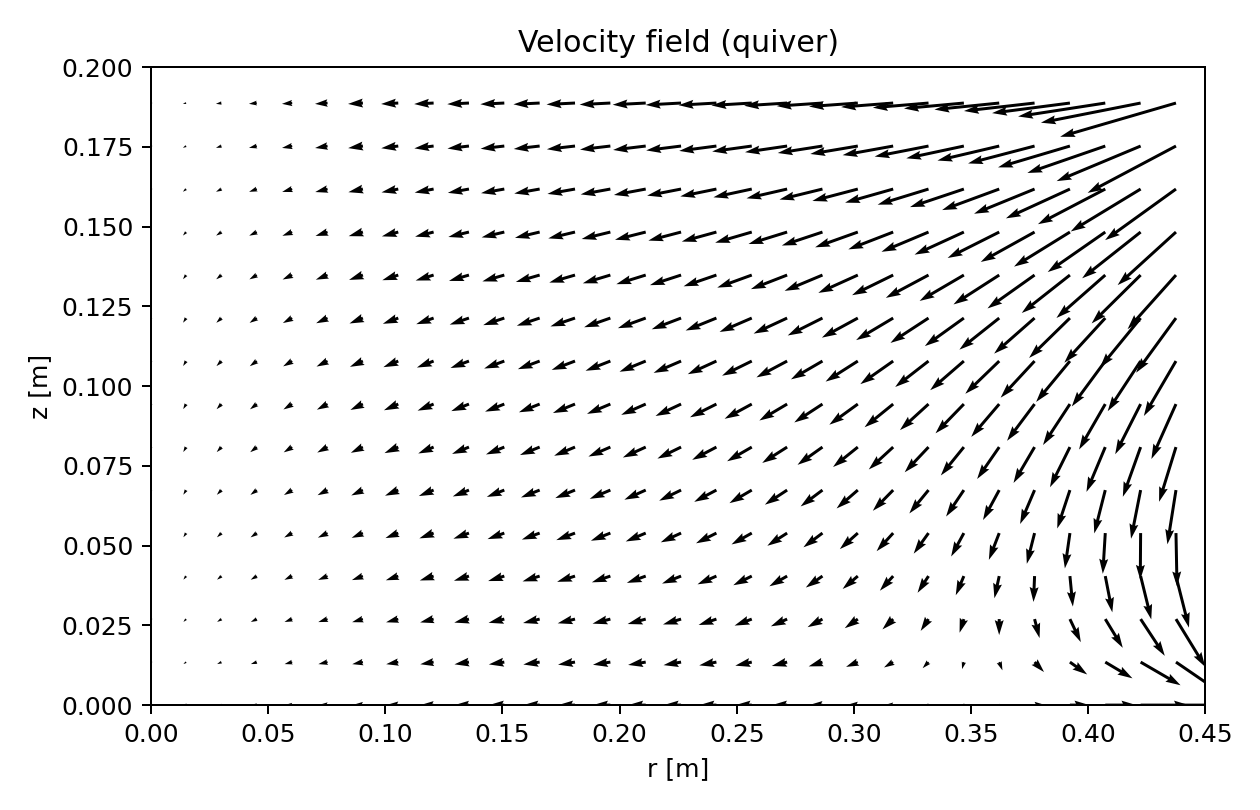
\includegraphics[width=0.95\linewidth]{../figs/quiver_velocity.png}
  \caption{Non-dimensional velocity field (quiver).
Vectors show $(\hat u,\,S\hat w)$ for isotropic visual scaling; the pattern reflects the rim-imposed sealing pressure from the downward curtain.}
  \label{fig:quiver}
\end{figure}\begin{figure}[H]
  \centering
  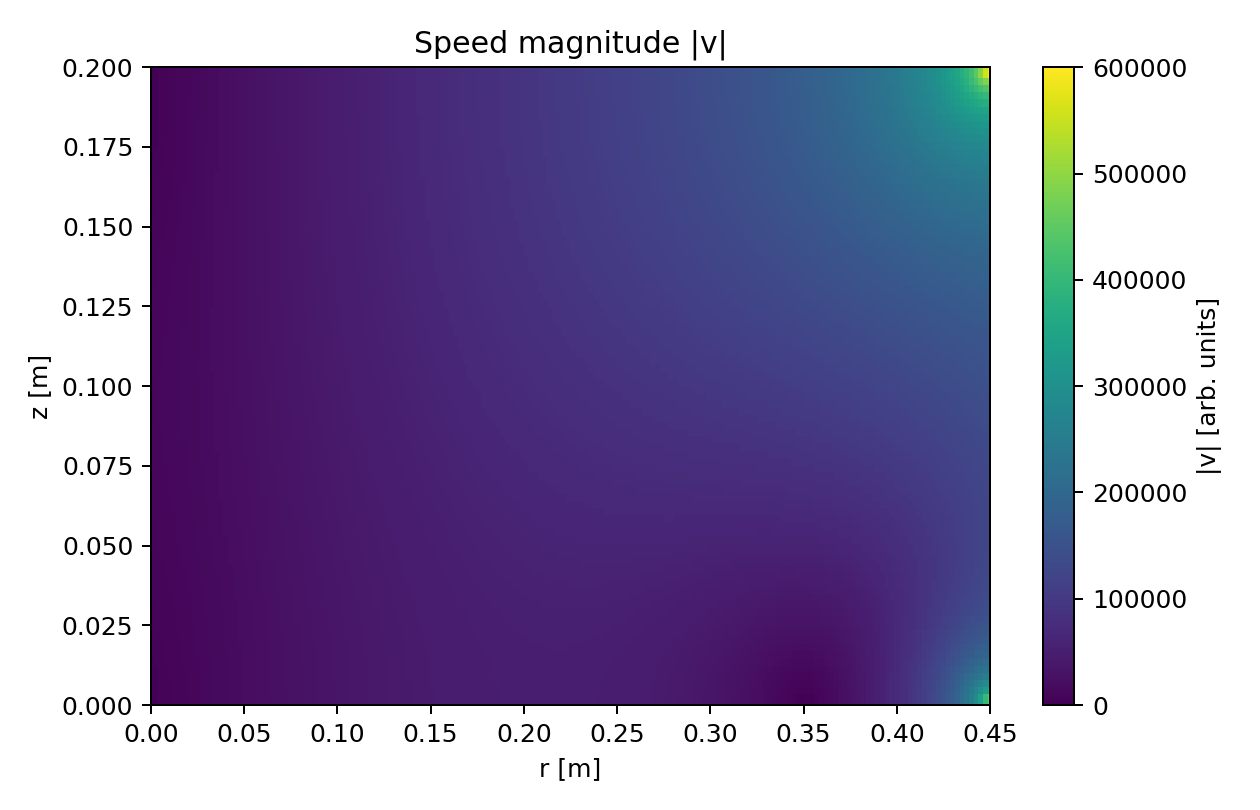
\includegraphics[width=0.95\linewidth]{../figs/cmap_speed.png}
  \caption{Colormap of the non-dimensional isotropic speed magnitude $\hat V_{\mathrm{iso}}=\sqrt{\hat u^{\,2}+S^{2}\hat w^{\,2}}$.}
  \label{fig:cmap_speed}
\end{figure}\begin{figure}[H]
  \centering
  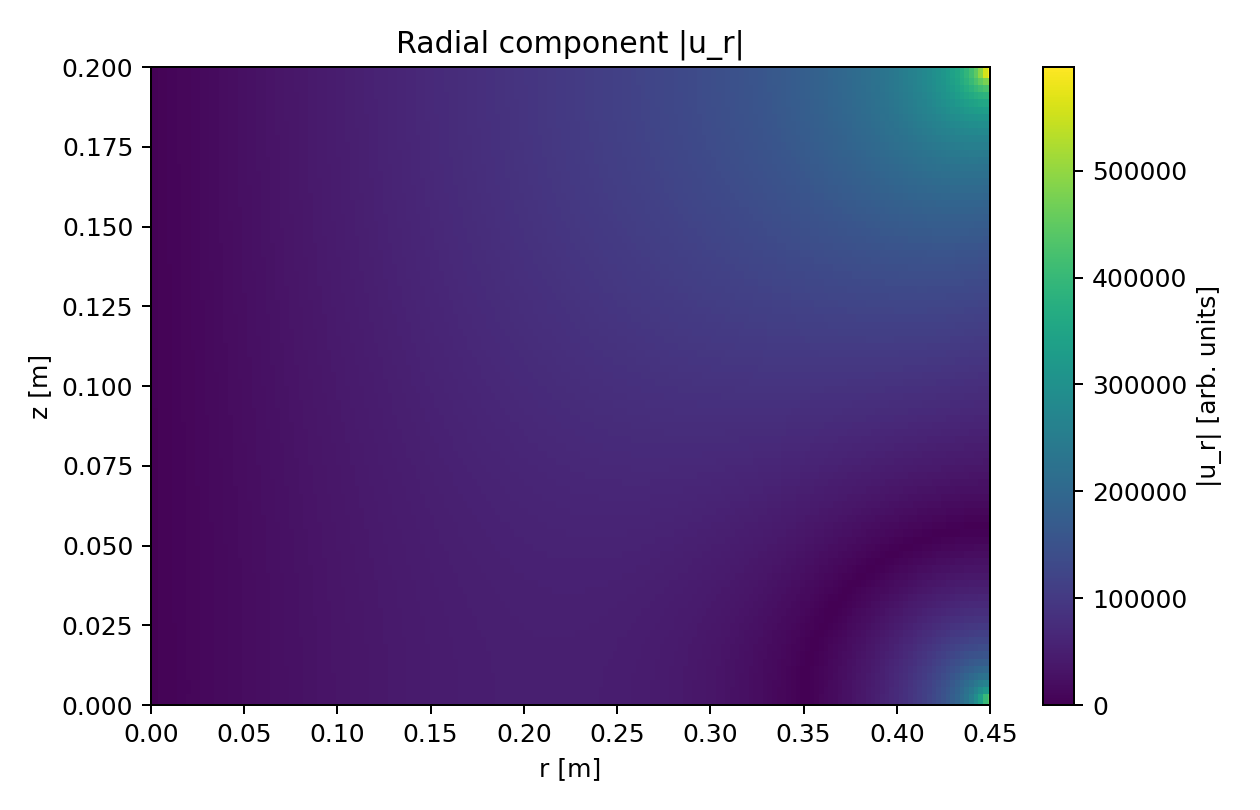
\includegraphics[width=0.95\linewidth]{../figs/cmap_ur.png}
  \caption{Colormap of the non-dimensional radial component magnitude $|\hat u|$.}
  \label{fig:cmap_ur}
\end{figure}\begin{figure}[H]
  \centering
  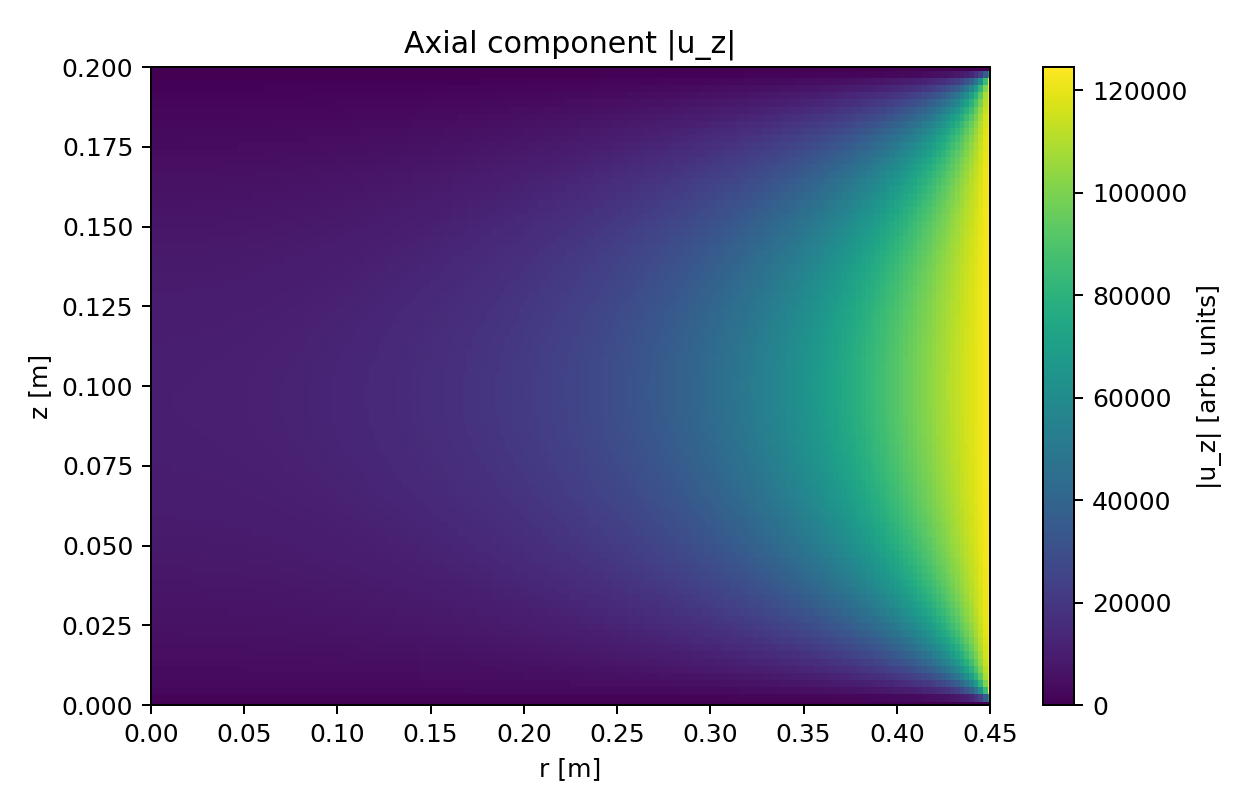
\includegraphics[width=0.95\linewidth]{../figs/cmap_uz.png}
  \caption{Colormap of the non-dimensional axial component magnitude $|\hat w|$.}
  \label{fig:cmap_uz}
\end{figure}\begin{figure}[H]
  \centering
  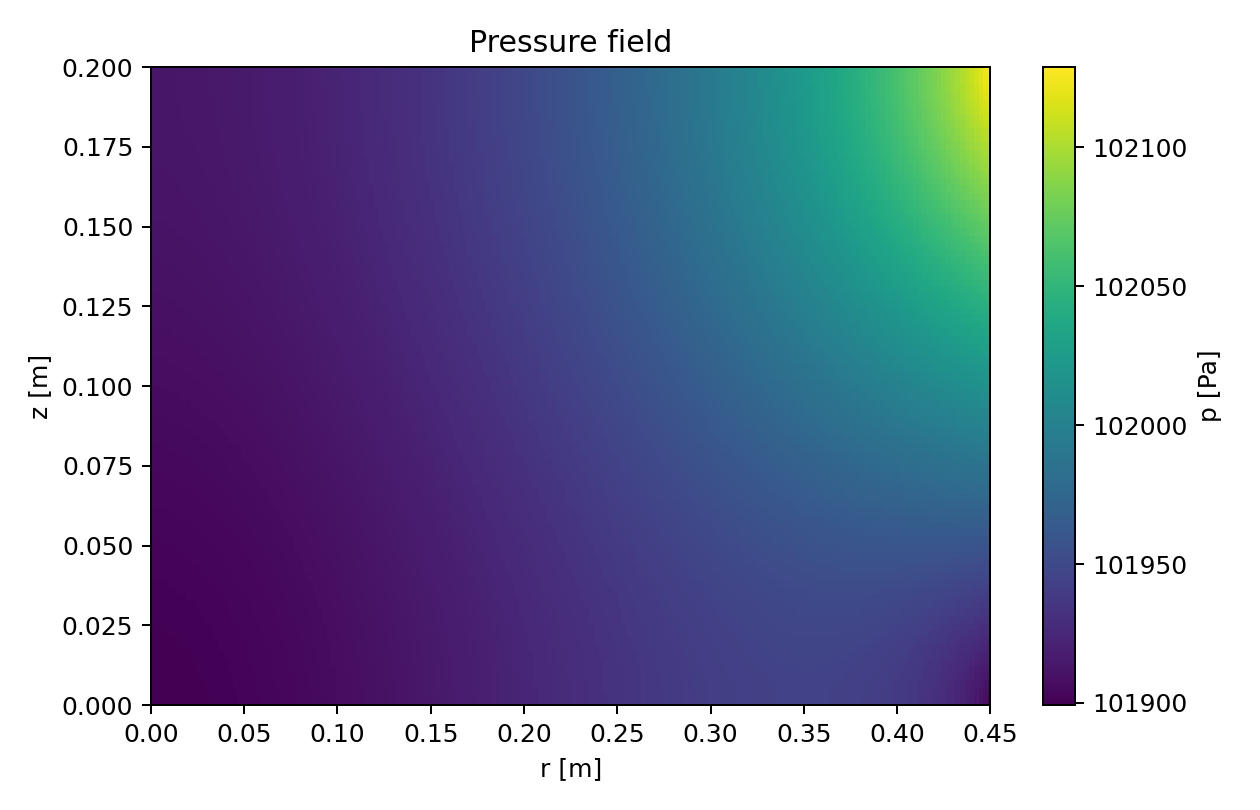
\includegraphics[width=0.95\linewidth]{../figs/cmap_pressure.png}
  \caption{Colormap of the non-dimensional pressure $\hat p$.}
  \label{fig:cmap_p}
\end{figure}

\section{Model Limitations and Planned Extensions}
\label{sec:model-limitations-and-planned-extensions}

The Darcy--Brinkman closure is an engineering reduction (effective permeability in a
free flow); $\alpha_r,\alpha_z$ should be calibrated against axisymmetric CFD.
The make-up jet is not imposed as a local BC in the core; it enters only via the
mass-balance closure. Thermal effects are neglected ($T=T_\infty$). The bypass parameter
$\beta$ is defined conceptually but not used yet in the code; it will be included together
with the automated shooting loop and power estimates.

\paragraph{Appendix: minimal rationale for the composite rim pressure.}
Consider a control volume hugging the rim over height $h$ and thickness $O(b)$.
A downward slot jet of density $\rho_j$ and speed $U_{\mathrm{out}}$ is deflected
into a radial wall-jet of speed $U_r(z)$ near the floor. A crude momentum balance
suggests a static build-up $\Delta p_{\mathrm{stat}}\sim \rho_j U_{\mathrm{out}}^2
\,\mathcal{O}(1)$ concentrated near $\zeta\!\to\!0$, while the resistance to
cross-flow (sealing) scales with the jet momentum flux impinging near the slot,
$\Delta p_{\mathrm{seal}}\sim \rho_j U_{\mathrm{out}}^2\,\mathcal{O}(1)$ for
$\zeta\!\to\!1$. The composite form
$\rho_j U_{\mathrm{out}}^2\,[\,C_p(1-\zeta)^n + C_s \zeta^m\,]$ is thus a
first-order surrogate capturing both effects with two tunable, dimensionless
coefficients $(C_p,C_s)$ and mild shape exponents $(m,n)$.

\paragraph{On the choice of $D_{m,\min}$.}
We take $D_{m,\min}$ from air-curtain literature (order $10^{-1}$) as a design parameter; in absence of calibration, $D_{m,\min}=0.2$ provides a conservative default.
Sensitivity to this parameter is reported without altering the solver or figures.

\section{Nomenclature}
\label{sec:nomenclature}

\begin{tabular}{@{}ll@{}}
\toprule
Symbol & Description \\ \midrule
$R_{\mathrm{tot}}$ & Total radius of the disc \\
$R^{-}$ & Inner radius of the leakage ring ($R^{-}=R_{\mathrm{tot}}-w$) \\
$w$ & Width of peripheral leakage region \\
$h$ & Hovering height (disc--ground gap) \\
$h_{\mathrm{eff}}$ & Effective sealing height at rim \\
$b_0$ & Slot thickness at injection (plane jet width) \\
$b(z)$ -- effective local width of the curtain slot or equivalent jet region as a function of $z$ \\
$U_{\mathrm{out}}$ & Outer jet velocity \\
$\rho_j$ & Density of outer jet \\
$\rho$ & Density in the core region \\
$p,p_0,p_c$ & Local, ambient, and cushion pressures \\
$T,T_\infty$ & Local and ambient temperatures \\
$\mu$ & Dynamic viscosity of air \\
$R_g$ & Specific gas constant of air \\
$W$ & Payload supported by cushion \\
$\kappa_r,\kappa_z$ & Effective permeabilities (radial/axial) \\
$\alpha_r,\alpha_z$ & Dimensionless permeability coefficients \\
$u,w$ & Velocity components (radial, vertical) \\
$\Delta p$ & Rim pressure increment \\
$\Pi_{\mathrm{edge}}$ & Dimensionless rim pressure amplitude \\
$\mathcal{A}$ & Permeability anisotropy parameter \\
$\hat r,\hat z,\hat p$ & Dimensionless coordinates and pressure \\
$\hat u,\hat w$ & Dimensionless velocity components \\
$S$ & Velocity anisotropy ratio $S=(\alpha_z/\alpha_r)(R_{\mathrm{tot}}/h)$ \\ $D_m$ & Deflection modulus (momentum index) $\rho U_0^2 b_0/(\Delta P\,H)$ \\
$D_{m,\min}$ & Minimum deflection modulus for sealing \\
$H$ & Effective curtain height \\
$s$ & Jet spreading parameter ($\approx0.06$--$0.09$) \\
$\Delta P_{\max}$ & Maximum sustainable pressure difference \\
$q(r)$ & Mass flow per unit circumference in wall-jet model \\
$m(r)$ & Momentum flux per unit circumference in wall-jet model \\
$\delta_t$ & Wall-jet thickness at turning radius $r_t$ \\
$r_t$ & Effective turning radius of the outer jet on the ground \\
$U_c(r)$ & Local characteristic velocity of the wall-jet at radius $r$\\
\bottomrule
\end{tabular}

% =====================================================

% --- Added notation for outer-jet seal model ---
\paragraph{Additional symbols.}
\begin{tabular}{ll}
\(r_t\) & effective turning radius of the outer jet \\
\(U_{\mathrm{out}}\) & injection speed of the outer (vertical) jet \\
\(A_{\mathrm{slot}}\) & outlet area of the outer jet \\
\(K_{\mathrm{turn}}\) & momentum loss coefficient at turning (impingement) \\
\(\delta\), \(\delta_t\), \(\delta_s\) & wall-jet thickness (generic / at \(r_t\) / at \(r_-\)) \\
\(U_c(r)\) & characteristic wall-jet speed \\
\(q(r)\), \(m(r)\) & mass and momentum per unit circumference \\
\(E\) & entrainment coefficient \\
\(C_f\) & wall friction coefficient, \(C_f=C_{f0} Re_\delta^{-1/5}\) \\
\(k_e\) & wall-jet thickness growth rate \\
\(w_s\) & seal strip width, \(w_s=\lambda\,\delta_s\) \\
\(\delta_p\) & effective thickness for pressure work in the seal strip \\
\(\Delta p\) & pressure jump between core and ambient
\end{tabular}


\end{document}